\chapter{The Maple Environment}
\label{chp:maple_environment}			

\section{Execution Groups}
\label{sec:execution_groups}

Maple input is used for computations and must use recognizable commands. Maple output gives the result of the computation after hitting the Enter key. Together, Maple input and output are called an \textit{execution group}.
\begin{itemize}
\item Place a new execution group after the current line with the 
\includegraphics[width=0.05\textwidth]{tutorials/figures/new_input.PNG} button.
\item Place a new execution group after the current line with Ctrl+J.
\item Place a new execution group before the current line with Ctrl+K.
\end{itemize}
Maple input is preceded by the $>$ character (sometimes called a "carrot"). Maple output is displayed in the centre of the following line.

\begin{marginfigure}
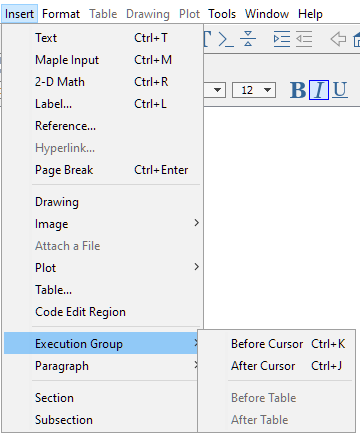
\includegraphics[scale=0.5]{tutorials/figures/InsertInput.png}
\caption{Using the Insert menu to include a new Maple execution group.}
\end{marginfigure}

\begin{maplegroup}
\begin{mapleinput}
\mapleinline{active}{1d}{2 + 2;
}{}
\end{mapleinput}
\mapleresult
\begin{maplelatex}
\mapleinline{inert}{2d}{4}{\[\displaystyle 4\]}
\end{maplelatex}
\end{maplegroup}
\begin{maplegroup}
\begin{mapleinput}
\mapleinline{active}{1d}{8 / 2;
}{}
\end{mapleinput}
\mapleresult
\begin{maplelatex}
\mapleinline{inert}{2d}{4}{\[\displaystyle 4\]}
\end{maplelatex}
\end{maplegroup}

If at any point you wish to correct a previous Maple input line, you may simply go back to that line and modify it. However, there will be no change to the output until you hit Enter. You do not need to be at the end of the line in order to run it.

You may wish to have more than one calculation or command on a single Maple input. For more information on this, see Tutorial \ref{chp:basics_of_maple_syntax} on page \pageref{chp:basics_of_maple_syntax}.

\section{Paragraphs}
\label{sec:paragraphs}

\begin{marginfigure}
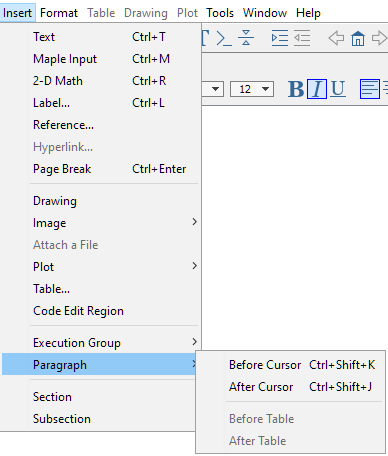
\includegraphics[scale=0.5]{tutorials/figures/InsertParagraph.png}
\caption{Using the Insert menu to include a new text paragraph.}
\end{marginfigure}

\textit{Paragraphs} are used for text, rather than for computation. Hitting Enter simply creates a new line of text and does not try to display a result.
\begin{itemize}
\item Create new text after the current line with the 
\includegraphics[width=0.04\textwidth]{tutorials/figures/new_text.PNG} button.
\item Create new text after the current line with Ctrl+Shift+J.
\item Create new text before the current line with Ctrl+Shift+K.
\end{itemize}

\section{Deleting Inputs}
\label{sec:deleting_intputs}

\marginnote{It's a good habit to delete unnecessary Maple inputs.}
Delete a section of Maple Input or Text using Ctrl+Delete. You will notice that hitting backspace will not delete a section by default.

\section{Three Font Styles}
\label{sec:three_font_styles}

There are two font styles that are commonly used in execution groups.
\begin{itemize}
\item ``2D Math" (the default in modern versions)
	\begin{itemize}
	\item In this mode, mathematical expressions are formatted nicely, as one would write them on paper. 
	\item Text will appear in \textit{italic}, with the exception of common mathematical functions and constants.
	\item An example of an expression in 2D Math: \[\displaystyle {\frac {{x}^{5}}{{\rm e}^{x}+\sin \left( x \right) }}. \]
	\item Switch to 2D Math using Ctrl+R.
	\end{itemize}
	\marginnote[-2cm]{While 2D Math has the advantage of looking prettier, it often treats spaces as multiplication and it doesn't always treat brackets as multiplication when desired. Maple Input causes fewer issues with how Maple interprets what has been typed, but it often requires the use of many more parenthesis. This lab manual will make frequent use of Maple Input for clarity, but you will likely use 2D Math for most of your exercises.}
\item ``Maple Input" (the default for old versions)
	\begin{itemize}
	\item In this mode, mathematical expressions are displayed inline, with no additional formatting. 
	\item All text is shown in \texttt{monospaced font}.
	\item The above expression in Maple input: 
		\begin{verbatim}
		x^5/(exp(x)+sin(x))
		\end{verbatim}
	\item Switch to Maple Input using Ctrl+M.
	\end{itemize}
\end{itemize}
Finally, paragraphs use a third style of font.
\begin{itemize}
\item ``Plain Text"
\marginnote{It can be useful to switch to 2D Math in paragraphs for an expression or equation, then switch back to text afterwards.}
	\begin{itemize}
	\item In this mode, mathematical expressions are displayed inline, with no additional formatting. 
	\item All text is shown in a standard font, such as this line.
	\item Switch to Plain Text using Ctrl+T.
	\end{itemize}
\end{itemize}

\section{Using Sections}
\label{sec:using_sections}

\textit{Sections} are groups of one or more execution groups or paragraphs that are indented together. At the top of a section, you can create a section title. An arrow to the left of the title will allow you to expand or collapse that section. Subsections may be created inside other sections.

\begin{itemize}
\marginnote{You may wish to highlight several execution groups or paragraphs with the mouse before combining them into one section.}
\item Use the 
\includegraphics[width=0.1\textwidth]{tutorials/figures/new_section.PNG} buttons to create or remove sections.
\item Use Ctrl+. to enclose input in a section.
\item Use Ctrl+, to remove any section enclosing an input.
\end{itemize}

\section{Palettes Toolbar}
\label{sec:palettes_toolbar}

You can open or close the palettes toolbar by clicking on the black arrows at the left side of the page.
\begin{figure}
\adjincludegraphics[width=0.495\textwidth]{tutorials/figures/palettes1.png}\hspace{.2cm}
\adjincludegraphics[width=0.505\textwidth]{tutorials/figures/palettes2.png}
\caption{Opening and closing the palettes toolbar.}
\end{figure}

With the palettes toolbar open, you can see several palettes that are available. These can be used to quickly access common operations and procedures by clicking on the appropriate buttons. Each palette can be expanded or closed. The Expression palette is especially useful for common functions.

\begin{marginfigure}
\centering
\adjincludegraphics[scale=0.6,trim={0 {.3\height} 0 0},clip]{tutorials/figures/palettes3.png}
\caption{The first few default palettes expanded.}
\end{marginfigure}
